
\documentclass[a4paper,twoside,12pt,titlepage]{article}

\usepackage[ngerman]{babel}
\usepackage[utf8]{inputenc}
\usepackage{a4wide}
\usepackage{lmodern}
\usepackage{graphicx}
\usepackage{amsmath}
\usepackage{amsfonts}
\usepackage{eurosym}
\usepackage{pdfpages}
\usepackage[condensed,math]{iwona}
\usepackage[T1]{fontenc}

\begin{document}
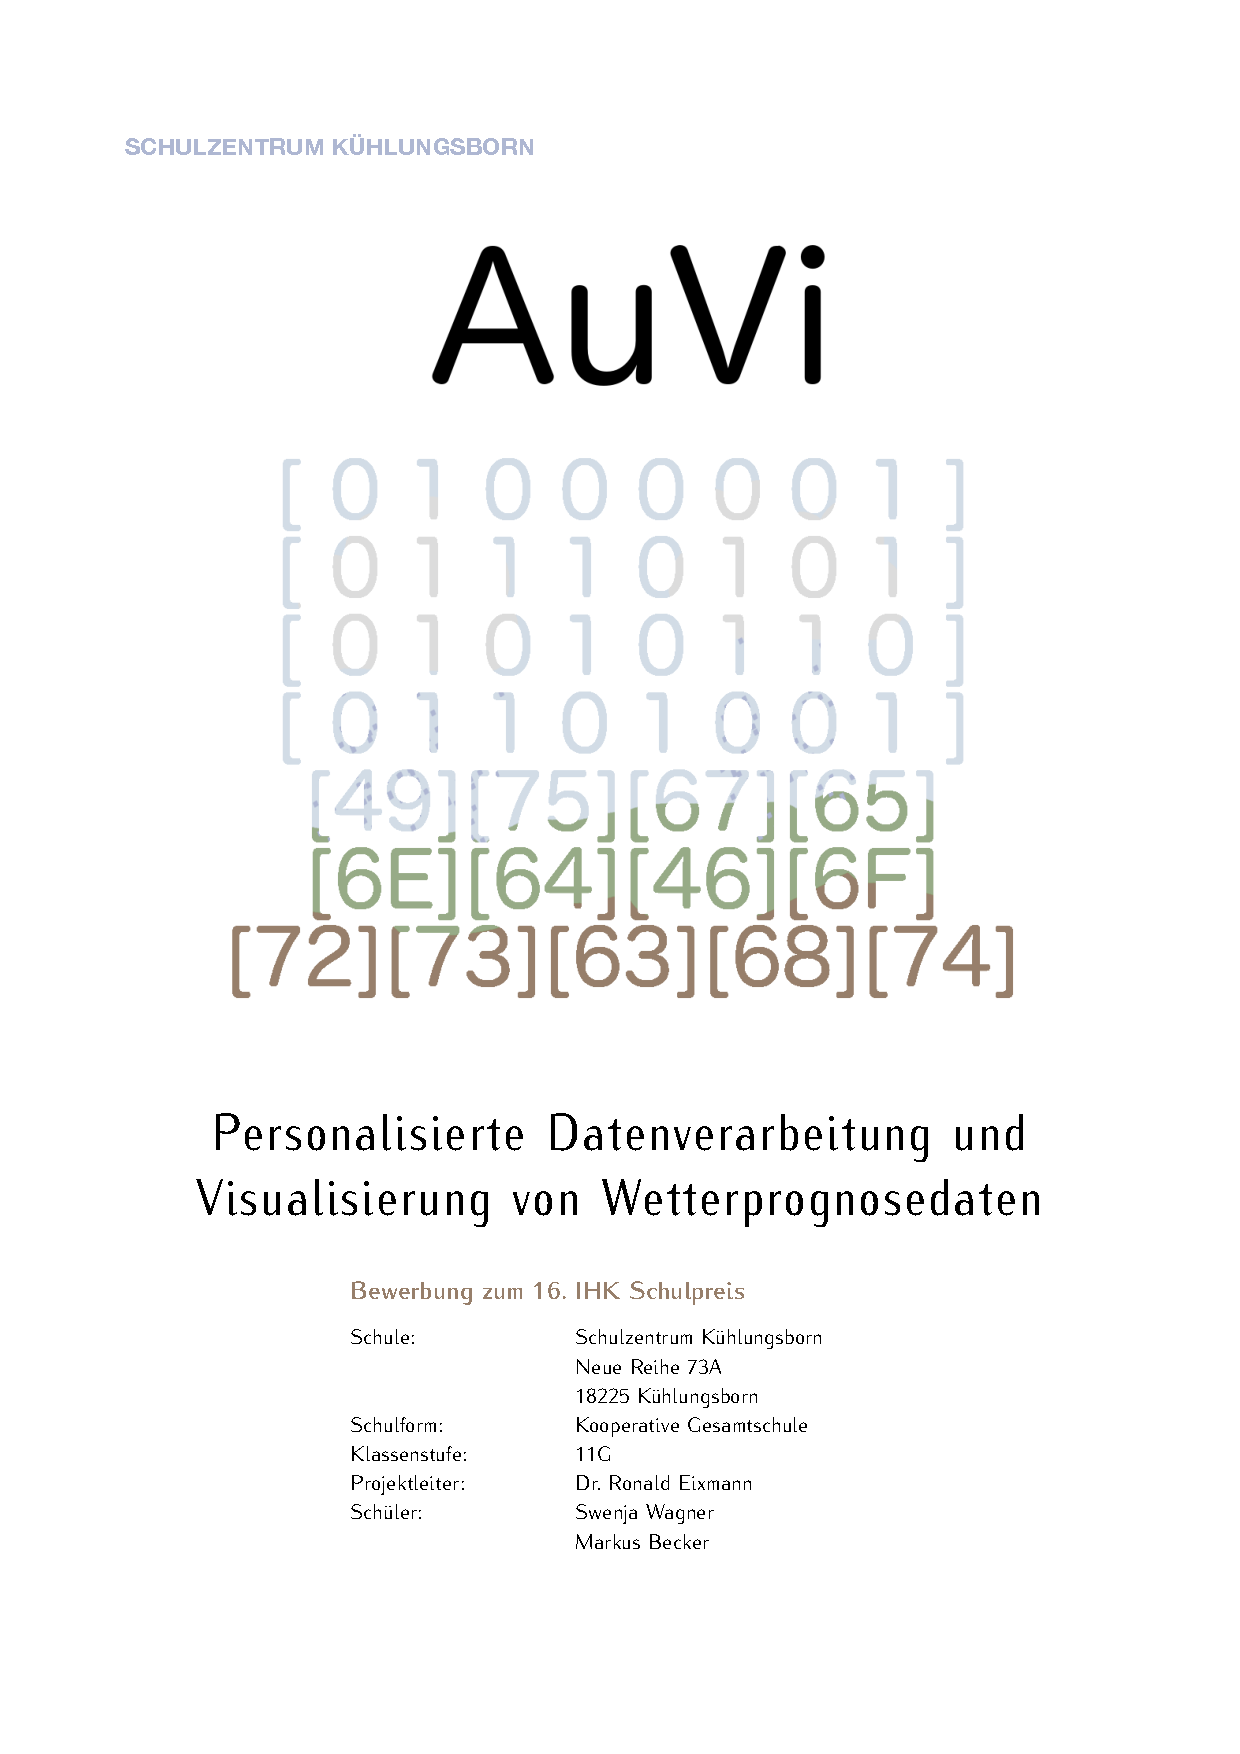
\includepdf{auvi_schulpreis_deckblatt.pdf}
\pagestyle{empty}
\tableofcontents
\thispagestyle{empty}
\pagestyle{plain}
\newpage

\paragraph{Abstract}
$ $\\
Wetterprognosen beziehen sich oft vor allem auf große Städte und markante Punkte. Sucht man jedoch eine Präzise Vorhersage für einen kleinen Ort oder in einer gewissen Höhe kann es schwierig werden. Daher haben wir ein Programm entwickelt, das für jeden beliebigen Punkt der Erdatmosphäre eine Prognose für die kommenden zehn Tage darstellt. Dabei hat der Nutzer volle Kontrolle über die Darstellung und die Parameter.\\
Dies ermöglicht diverse Nutzungsbereiche von Frühwarnsysteme für Extremsportler oder Arbeiter über den Segler und Flugzeugpiloten bis hin zu Wissenschaftlern, die so Zugriff auf alle Parameter verschiedenster Quellen erhalten. Wir erhoffen uns, dass wir unser System auch bald in Hotels und Restaurant einsetzen können.

\section{Zielsetzung}
\subsection{Visualisierung}
Unser Projekt handelt von der gezielten Visualisierung von Wetterprognosedaten. Wir wollen in der Lage sein für jeden beliebigen Punkt auf der Erde eine Grafik mit Interpretation anzubieten.\\ Bei dieser Grafik sprechen wir von einem Funktions- oder Konturplot, der für bzw. um den Ort einen oder mehrere Parameter visuell veranschaulicht.
\subsection{Verbreitung}
Die von uns erzeugten Grafiken sollen zusammen mit einer automatisiert generierten Interpretation auf einer frei verfügbaren Website veröffentlicht werden. Wir wollen auch die Möglichkeit bieten, durch ein Konto personalisierte, angepasste Bilder anfordern zu können. Diese Kontos sind unser Ansatz unser Projekt selbst zu finanzieren.\\
Unser System soll auch in Hotels, Ferienwohnungen und evtl. sogar Restaurants Anwendung finden. Da diese Einrichtungen oft auf ein u.a. einheitliches Farbschema Wert legen, sollen die Grafiken auch für das entsprechende Klientel angepasst sein. Der normale Besucher interessiert sich eher für Temperatur, Wind, Regenwahrscheinlichkeit und Bewölkung. Wir sind aber auch in der Lage meteorologisch komplexere Parameter zu visualisieren. So können wir Ergebnisse liefern, wenn sich jemand für die aktuelle Ozonverteilung der Atmosphäre oder die Lufttemperatur in über 30.000 Kilometern Höhe interessiert.
\section{Durchführung}
\subsection{Arbeitsweise}
Dass Projektteam besteht aus Swenja Wagner und Markus Becker. Wir teilen uns die Aufgaben der Programmierung und Setzung unserer Arbeit. Zusammen bilden wir das Vortragsduo, und treten für unser Projekt in der Öffentlichkeit auf. Unser Projektleiter Dr. Ronald Eixmann, Diplom Meteorologe, unterstützt uns bei unserer Arbeit und steht uns mit Rat und Tat zur Seite. Er vermittelte uns auch die Grundlagen der Meteorologie. Einmal wöchentlich treffen wir uns um unsere Fortschritte abzusprechen und uns neue Schwerpunkte zu setzen.
\subsection{Technik}
Da wir ein sehr technisches Projekt bearbeiten, nutzen wir Computer und Laptops. Den Eigenanteil der Arbeit erledigen die Teilnehmer unseres Teams auf ihren privaten Laptops. Für die Zusammenführung unserer Ergebnisse und der Ausführung unseres Programmcodes nutzen wir zwei Raspberry Pi's, Mikrocomputer auf Linux-Basis die unser Programm ausführen können und wirtschaftlich sowie umweltbewusst durchgängig betrieben werden können.\\
Für den Betrieb und das umfangreiche Testen müssen wir diese Programme ausführen und Testdaten eingeben. So wählen wir verschiedene Orte der Welt aus und erzeugen regelmäßig Grafiken und überprüfen diese auf Korrektheit und versuchen weiterhin unsere Software und den Ablauf des Generierungsprozesses weiter zu optimieren.\\
Unsere Datenquelle für die Visualisierung ist der Amerikanische Wetterdienst. Wir nutzen das GFS (Global Forecast System) um an die aktuellen Wetterdaten zu gelangen. Es ist aus technischen Gründen nicht möglich selbst die Prognosedaten zu errechnen, da man dafür ein weltweites Netzwerk aus Wetterstationen, sowie anderen Messeinrichtungen benötigt. Zusätzlich müssen Supercomputer diese Daten dann auswerten und interpolieren.
\subsection{Angebot}
Unsere Ergebnisse werden auf lokalen HTML-Webseiten eingebunden, somit kann der Nutzer eines PC's mit eigener ,,AuVi'' (Automatisierte Visualisierung) Software die neuesten Ergebnisse ohne Probleme und ohne den Quellcode zu verstehen sofort und mit maximalen Komfort betrachten. Des weiteren kann diese Webseite mit der Gesamtheit der erzeugten Grafiken ohne Abänderungen auch direkt im Internet veröffentlicht werden. So testen wir unsere eigenen Ergebnisse. 
\section{Ergebnis}
\subsection{,,AuVi''-Programm}
Das Ergebnis unserer Arbeit haben wir ,,AuVi'' getauft. Es ist ein Programm zur Generierung von Grafiken. Dieses haben wir in zwei Sprachen geschrieben um es auf verschiedensten Unix-Systemen ausführen zu können. Zuerst schrieben wir es in BASH und später erstellten wir ein Python Modul-Paket, das all unsere Routinen, gut dokumentiert, verpackt. In diesen Routinen greifen wir auf zwei fremde, öffentlich frei verfügbare Programme zurück, für die wir selbst wieder Skripte geschrieben haben, damit sie automatisiert die von uns gewünschten Aufgaben ausführen. Diese Programme sind GrADS (Grid Analysis and Display System), welches uns hilft die Datensätze des Amerikanischen Wetterdienstes auszulesen und ImageMagick, welches wir nutzen um unsere Grafiken in leichter verständliche Videos umzuwandeln.\\
Um nur kurz auf die ganz informatorischen Eigenschaften unseres Programms einzugehen: es benötigt ca. 1 GB RAM um die Datensätze zuverlässig zu verarbeiten, eine stabile Internetverbindung zum Start, um die Datensätze abzurufen, und die Laufzeit in Prozessorminuten beläuft sich auf unseren Testmaschinen auf: $$T(\overbrace{a}^{\text{Anzahl Zeitdaten}},\overbrace{o}^{\text{Anzahl Orte}}, \overbrace{p}^{\text{Anzahlt Parameter}})=(a\cdot o\cdot p)\cdot\underbrace{0.021+0.0025}_{\text{Hardwarekonstanten}}o\cdot a$$ $$T(a,o,p)\in O(a,o,p)=(a\cdot o \cdot p)$$Am Beispiel mit 72 Zeitdaten in Stunden, 50 beliebigen Orten und 5 verschiedenen Parametern z.B. Luftdruck, Temperatur, Wassersäule (aus der sich die Regenwahrscheinlichkeit ausrechnen lässt), Windstärke und Windrichtung oder Ozon haben wir dann $T(72,50,5)\approx 387\text{min}\approx 6.5\text{h}$. Für uns bedeutet das, dass das Generieren von Grafiken für die nächsten 3 Tage im stündlicher Genauigkeit für fünfzig Orte circa sechs Stunden benötigt\footnote{Der von uns genutzte Rechner ist ein $\sim$ 40 \euro$ $ Raspberry Pi 2.} .\\ Deshalb generieren wir die Siebentagevorschau seltener und visualisieren die zeitlich näherliegenden Ergebnisse öfter. Die Ergebnisse müssen abgespeichert werden und nehmen für die selben Testdaten etwas über 5 GB ein. Sie sind aber direkt für den Gebrauch im Web komprimiert und stehen in der von uns vorhergesehenen Struktur zur Verfügung.
\subsection{Webpräsenz}
Die Website wird dynamisch während der Visualisierung mit erzeugt und bindet sofort alle aktuellen Grafiken ein. Dies beinhaltet alle Orte mit dazugehörigen Parametern. Nun können wir die Orte und Parameter auf verschiedene Rechner verteilen und für die Webpräsenz die Daten auf einem Rechner zusammenfließen lassen. So können wir dem Nutzer einen ganz individuellen Zugriff auf unsere und die Quelldaten ermöglichen. Des weiteren haben wir ein weiteres Anzeigeformat. Bei diesem Handelt es sich um eine Vollbildanwendung die immer die neusten Grafiken für eine von uns festgelegte Menge von Ort- und Parameterpaaren enthält. Beim Erzeugen dieser Grafiken wird zeitgleich eine Tabelle in Textform erzeugt, welche die markanten Wetterdaten der Prognose enthält. Diese Wetterdaten sind Höchsttemperatur, Niederschlagswahrscheinlichkeit und Bewölkung.

\newpage
$ $\\$ $
\Large{Quellen}
\\
\\
\small{
Datenserver \& GFS:\\
http://www.ncdc.noaa.gov/data-access/model-data/model-datasets/global-forcast-system-gfs \\(13.01.2015)\\\\
Kühlungsborner Seewetterstation:\\
http://seewetterstation-kborn.de/ \\(15.01.2015)\\\\
GrADS-Website:\\
http://iges.org/grads/ \\(15.01.2015)\\\\
Imagemagick:\\
http://www.imagemagick.org/ \\(15.01.2015)\\
}
\\
\\
\\
\Large{Selbstständigkeitserklärung}\\
\\
\small Hiermit erklären wir, dass wir die vorliegende Arbeit selbständig angefertigt, nicht anderweitig zu Prüfungszwecken vorgelegt und keine anderen, als die angegebenen Hilfsmittel verwendet haben. Zudem waren alle verwiesenen Webseiten zum Zeitpunkt der Linksetzung gültig und erreichbar. Wörtlich und sinngemäße Übernahmen aus anderen Werken sind als solche gekennzeichnet.
\\ 



\end{document} 
